\documentclass{standalone}
\usepackage{tikz}
\usepackage{ctex,siunitx}
\setCJKmainfont{Noto Serif CJK SC}
\usepackage{tkz-euclide}
\usepackage{amsmath}
\usetikzlibrary{patterns, calc}
\usetikzlibrary {decorations.pathmorphing,decorations.pathreplacing,decorations.shapes,}
\begin{document}
\small
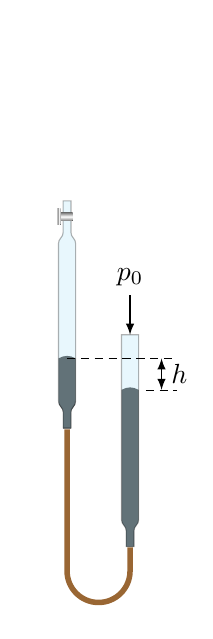
\begin{tikzpicture}[>=latex,scale=1.0]
  \useasboundingbox(-0.5,1.9)rectangle(1.5,-5.5);
  \fill[darkgray](-0.108,-2.3)--++(0,-0.55)arc(180:225:0.1)arc(45:0:0.1)--++(0,-.2)--++(0.1,0)--++(0,0.2)arc(180:135:0.1)arc(-45:0:0.1)--++(0,0.55)to[bend right]cycle;
  \fill[cyan!30,opacity=0.3,draw=black](0.05,-0.3)--(-0.05,-0.3)--++(0,-0.4)arc(0:-45:0.1)arc(135:180:0.1)--++(0,-2)arc(180:225:0.1)arc(45:0:0.1)--++(0,-.2)--++(0.1,0)--++(0,0.2)arc(180:135:0.1)arc(-45:0:0.1)--++(0,2)arc(0:45:0.1)arc(225:180:0.1)--cycle;
  \fill[top color=gray,bottom color=gray,middle color=white](-0.08,-0.55)rectangle(0.07,-0.45);
  \fill[left color=gray,right color=gray,middle color=white](-0.12,-0.6)rectangle(-0.08,-0.4);
  \begin{scope}[xshift=0.8cm,yshift=-1.5cm]
    \draw[->](0,0)--++(0,-0.5)node[at start,above]{$p_0$};
    \fill[darkgray](-0.108,-1.2)--++(0,-1.65)arc(180:225:0.1)arc(45:0:0.1)--++(0,-.2)--++(0.1,0)--++(0,0.2)arc(180:135:0.1)arc(-45:0:0.1)--++(0,1.65)to[bend right]cycle;
  \fill[cyan!30,opacity=0.3,draw=black](-0.108,-0.5)--++(0,-2.35)arc(180:225:0.1)arc(45:0:0.1)--++(0,-.2)--++(0.1,0)--++(0,0.2)arc(180:135:0.1)arc(-45:0:0.1)--++(0,2.35)--cycle;
  \end{scope}
  \draw[brown!80!black,line width=0.7mm](0,-3.2)--++(0,-1.8)arc(180:360:0.4)--++(0,0.3);
  \draw[thin,<->](1.2,-2.3)--(1.2,-2.7)node[right,midway]{$h$};
  \draw[very thin, densely dashed] (0,-2.3)--(1.4,-2.3)(1.0,-2.7)--(1.4,-2.7);
\end{tikzpicture}
\end{document}